% Character table modulo 5. Columns are n = 0,1,2,3,4.
% psi(2) = i, so psi(4) = psi(2)^2 = -1 and psi(3) = psi(2)^3 = -i, since 3 \equiv 2^3.
% The Legendre row is the real character with value -1 at 2. Complex rows are coral.
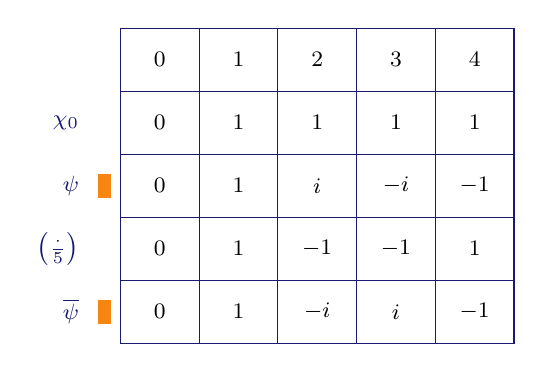
\begin{tikzpicture}[every node/.style={font=\footnotesize}]
  \draw[MidnightBlue] (0,0) rectangle (5.0,4.0);
  \foreach \x in {1,2,3,4} {
    \draw[MidnightBlue] (\x,0)--(\x,4.0);
  }
  \foreach \y in {0.8,1.6,2.4,3.2} {
    \draw[MidnightBlue] (0,\y)--(5.0,\y);
  }
  \node at (0.5,3.6) {$0$};
  \node at (1.5,3.6) {$1$};
  \node at (2.5,3.6) {$2$};
  \node at (3.5,3.6) {$3$};
  \node at (4.5,3.6) {$4$};
  \node[MidnightBlue,anchor=east] at (-0.40,2.8) {$\chi_0$};
  \node at (0.5,2.8) {$0$};
  \node at (1.5,2.8) {$1$};
  \node at (2.5,2.8) {$1$};
  \node at (3.5,2.8) {$1$};
  \node at (4.5,2.8) {$1$};
  \fill[BurntOrange] (-0.28,1.85) rectangle (-0.12,2.15);
  \node[MidnightBlue,anchor=east] at (-0.40,2.0) {$\psi$};
  \node at (0.5,2.0) {$0$};
  \node at (1.5,2.0) {$1$};
  \node at (2.5,2.0) {$i$};
  \node at (3.5,2.0) {$-i$};
  \node at (4.5,2.0) {$-1$};
  \node[MidnightBlue,anchor=east] at (-0.40,1.2) {$\bigl(\frac{\cdot}{5}\bigr)$};
  \node at (0.5,1.2) {$0$};
  \node at (1.5,1.2) {$1$};
  \node at (2.5,1.2) {$-1$};
  \node at (3.5,1.2) {$-1$};
  \node at (4.5,1.2) {$1$};
  \fill[BurntOrange] (-0.28,0.25) rectangle (-0.12,0.55);
  \node[MidnightBlue,anchor=east] at (-0.40,0.4) {$\overline{\psi}$};
  \node at (0.5,0.4) {$0$};
  \node at (1.5,0.4) {$1$};
  \node at (2.5,0.4) {$-i$};
  \node at (3.5,0.4) {$i$};
  \node at (4.5,0.4) {$-1$};
\end{tikzpicture}
